\documentclass[a4paper,10pt,onecolumn]{article}
\usepackage{graphicx,color,draftwatermark}
% \SetWatermarkText{v. 20121004}
% \SetWatermarkText{\includegraphics{moon1.eps}}
\usepackage{hyperref}
\hypersetup{colorlinks=true, linkcolor=blue, filecolor=blue, urlcolor=blue}
\pagestyle{empty}
\sloppy
\usepackage[left=2.2cm,top=1.5cm,right=1.8cm,bottom=1.5cm,nohead,nofoot]{geometry}
\makeatletter
\def\@seccntformat#1{}
\makeatother

\begin{document}

\bigskip
\bigskip
\title{Thoughts on the WA$+$ practical implementation}
\author{Yann Chemin}
\maketitle

\section{Introduction}
How to think about geospatial science and data when engaging into a large area/time implementation such as the WA+?
This letter is trying to gather some particular points of interests.\newline

The surface World as defined by its landforms so far is 510.1 million km2. While some parts are not heavily 
colonized by human such as the cryosphere, others, like the equatorial region is densely populated. 
Obvious competition for natural resources apply in such a case, first of all water. An accounting of water
is a hope to rationalize when and where water is going and what is being done with it, if it is lost from the
natural resource {\bf bank} for the anthroposphere.\newline

Applicable conditions are the availability of methods to provide a rationalization mean, that should be address that WA+
itself.
Additionally, there must be scientific methods to provide measurements of each of the water incarnations studied 
along their lives in the geographical zone of constraints. It turns out that hydrosciences have already a vast 
amount of available methods for doing so, from field measurements, modeling to remote estimations. 
The conditions being there, what are the aspects that should be considered in term of implementation of a recipient
of water incarnations measurements into a {\it centrum} of appropriate holistic connectivity to abstract completely 
to the type of dimensions requirements for any of the four WA+ entities to properly converge into existence each time.
\newline

The actual level of field monitoring in the geographical areas of IWMI's interest is dramatically low, and if any 
available, it may be under governemental preemption. The task at hand is thus an analytical one in many cases where 
modeling and remote tools prevail. In some cases, they can even be combined to improve specific quantification.
This will be of course well integrated into the need of WA+ since it is based on natural and anthropogenic types and
their relation to water, separating sub- or surface.\newline

The {\it Centrum} is per se able to speak the models/sources languages and translating those into an abstracted form
that will inherently generate cohesion. From cohesion, elegance and maintenance co-exist. Thus, arises the generation
of transparent connectors from the water and the framework. Building a framework, would then be independent of the 
{\it Centrum}, and maintenance too. Thus, avoiding commonly known implementation failures.\newline

A framework such as this type is inherently multi-dimensional, and there is concern in implementing it in a safe way.
Obviously, missing information is the usual suspect, and how handle it for convergence of the interesting sheet is a
primordial topic. especially, if {\it when} is added to {\it where}. Other concerns are essentially about accuracy 
and uncertainty estimations from multi-dimensional and mixed sources, emerging through a single value in a sheet.
Of less scientific importance is the user participation into the design of the framework interface.\newline

There is much to think about how to generate cohesion, abstract and connect water with a WA+ framework. 
Ample discussions of appropriate parties are a necessity to make a sound implementation. One can think of 
two sub parties on a first thought, the framework builders/users and the water information builders/maintainers.
In any case these sub-groups have also to be connected too.

\section{Implementation}
A proposed implementation is described here. Data products available as International Public Goods (like MOD16 ET, 
or from models like PERSIANN) will be sought to get started. As those datasets are fit in the {\it centrum} database,
a first implementation of the GIS plugin to prepare, quality check and analyze the WA$+$ components. The output of the
GIS plugin will be validated sheets appropriate for web dissemination. An secondary level analysis will be policy briefs
as per analysis of the produced sheets.
\newline
As the quality of the input improves, their will be a need to reassess uncertainty levels within the GIS plugin so that 
the WA$+$ procedure converges to more appropriate accuracy levels, especially when reaching scale limits of analysis.
\begin{center}
 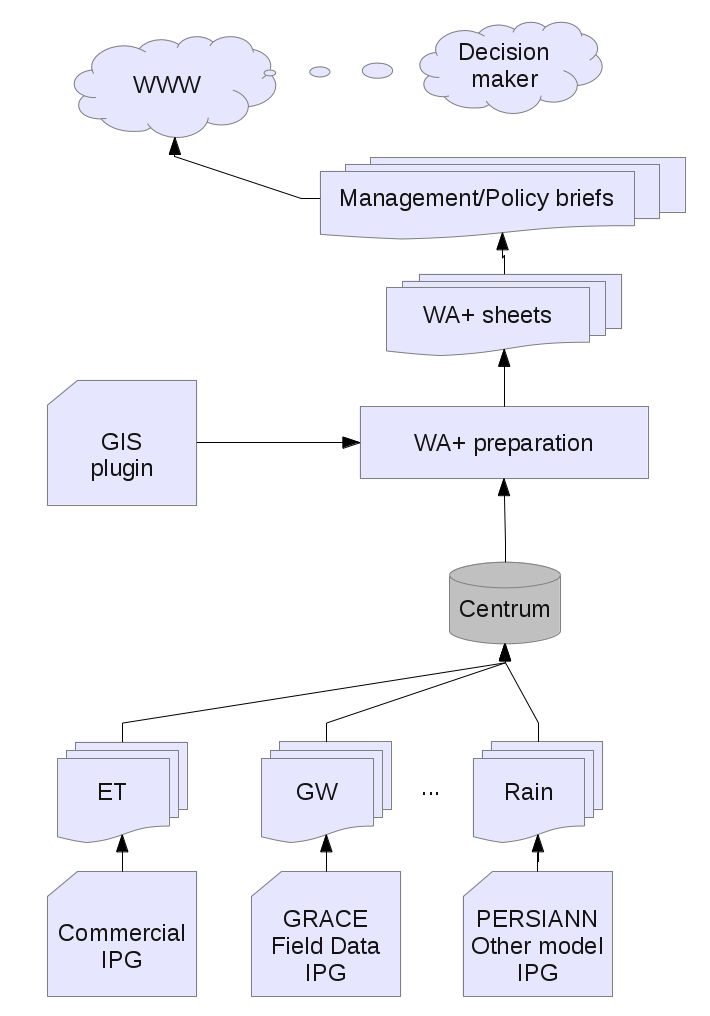
\includegraphics[scale=0.8,keepaspectratio=true]{./20130426_WAp_arch.png}
 % 20130426_WAp_arch.png: 644x936 pixel, 96dpi, 17.04x24.76 cm, bb=0 0 483 702
\end{center}

\section{GIS plugin}
Advanced Water Accounting (r.watacca) is a GIS plugin that enables a user to compute different versions of water accounting
(Molden, 1997; Karimi, 2013) on a geographical area of interest (water basin, irrigation system, etc). It produces 
actor-based report sheets (web-style, pdf, or spreadsheet software formats) for all of the possible water accounting
indicators permitted by input data. In case the user does not have all data and would like some to be estimated from 
online sources (needs internet), then r.watacca will search online solutions to plug into the missing paramaterization
set to estimate the best solution to the user's need.

\section{Central database (centrum)}
The online repository will have to deal with a lot of different and large datasets, rasdaman 
(\href{http://www.rasdaman.org}{www.rasdaman.org}) and postGIS (\href{http://postgis.net/}{postgis.net}) are both suitable
for such needs. Connectivity from client user to import IWMI standard sets is possible if user is missing some parameters 
and IWMI has it stored online (see GIS plugin section).

\section{Intput parameters}
Because of the highly integrative nature of such approach to performance evaluatuation, water accounting requires many 
different sources of data, both in high dimensionality and accuracy (high parametric sensitivity deviation). This is 
requiring the state of the art of science for each input parameter. Wherever the user may have its own dataset,
it will be preferred to use it with the GIS plugin. For parameters not measured, IWMI will have its set of estimated
parameters, regionally estimated from its various scientific sources, available as an online GIS file download (independent
of the GIS plugin), or a centrum database connection (from within the GIS plugin). \newline

The data set will invariably have different dimensionality. We propose to set two standards in time and space.
\begin{itemize}
 \item Time: daily and monthly
 \item Space: 100m and 1km
\end{itemize}
This will have most of the dimensions of interest addressed, while respecting most of the scienctific sources.



\end{document}
